\documentclass[10pt,a4paper,landscape]{article}
\usepackage[utf8]{inputenc}
\usepackage[czech]{babel}
\usepackage[T1]{fontenc}
\usepackage{amsmath}
\usepackage{amsfonts}
\usepackage{amssymb}
\usepackage{graphicx}
\usepackage{multicol}
\usepackage[left=1cm,right=1cm,top=0.2cm,bottom=1cm]{geometry}
%\usepackage{enumerate}

\author{Ondřej Zelenka}
\setlength{\columnsep}{1cm}
\begin{document}
\pagestyle{empty}
\textbf{\center\LARGE Závěrečná paralympiáda starších, LMFS 2023: Závěrečný deathmatch}
\vfill

\begin{multicols}{2}[]

\section{Teplý drát (11 bodů)}
Prof. Grill plave ve Slapech mezi termobójemi pod válcovým měděným vodičem, jehož konce leží na špičkách bójí. Odpor vodiče při teplotě $0^\circ\mathrm{C}$ je $10\,\Omega$, bóje ovšem zahřívají jeden konec na $34^\circ\mathrm{C}$ a druhý na $380^\circ\mathrm{C}$. Průběh teploty vodičem se ustálí v lineárním tvaru. Určete celkový odpor vodiče.

\begingroup\renewcommand\thesection{\arabic{section}.}
\section{kosmická rychlost (10 bodů)}
Určete 2. kosmickou rychlost, tedy nejmenší počáteční rychlost, se kterou hmotný bod (např. vesmírná loď) dokáže z povrchu Země setrvačností docestovat neomezeně daleko. Zanedbejte odpor atmosféry apod. Potenciální energie gravitační síly je
\begin{equation}
E_p\left(\vec{r}\right) = -G\frac{m_1m_2}{\left|\vec{r}\right|} ~.
\end{equation}
\endgroup

\section{Elektrosilná interakce (12 bodů)}
Ondra se rozhodl postavit urychlovač částic, aby v něm proton-protonovými srážkami vytvořil Higgsův boson, na což potřebuje celkovou energii srážky alespoň $125\,\mathrm{GeV}$. Postavil trubici kolem rovníku Země a na zakřivení trajektorie protonů využívá gravitační sílu a zemské magnetické pole, které na rovníku míří přímo na sever (vodorovně). Je ovšem pro tento účel příliš slabé a inspirován filmem The Core, Ondra roztáčí zemské jádro. Jak silné magnetické pole potřebuje, aby udrželo urychlené protony v trubici?

\section{Otáčení (8 bodů)}
Mějme vektorové pole dané rovnicí
\begin{equation}
\vec{E}\left(x,\, y,\, z\right) = \left(\frac{2xy}{z},\, \frac{x^2}{z},\, -\frac{x^2y}{z^2} + e^z\right) ~.
\end{equation}
Rozhodněte, zda má potenciál, a pokud ano, určete jej. Pokud ne, nemusíte jej určovat.

\section{Deska v2.0 (12 bodů)}
Nekonečná rovinná deska o tloušťce $a$ je rovnoměrně nabita nábojem s objemovou hustotou $\rho$. Najděte intenzitu i potenciál (pozor, musí být spojitý!) v každém bodě jak vně, tak uvnitř desky.

\section{Odporný odporník (8 bodů)}
\begin{minipage}{0.65\linewidth}
Určete proudy ve všech větvích vyobrazeného obvodu. Elektromotorická napětí zdrojů jsou $U_1 = 8\,\mathrm{V}$, $U_2 = 4\,\mathrm{V}$ a $U_3 = 2\,\mathrm{V}$, a odpory rezistorů jsou $R_1 = 12\,\Omega$, $R_2 = 6\,\Omega$ a $R_3 = 8\,\Omega$.
\end{minipage}
\hspace{0.05\linewidth}
\begin{minipage}{0.3\linewidth}
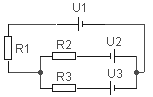
\includegraphics[width=\textwidth]{obvod.png}
\end{minipage}

\section{Nabitý prostor (8 bodů)}
Spočtěte objemové rozložení náboje v prostoru, jehož elektrické pole má potenciál
\begin{equation}
\varphi\left(\vec{r}\right) = U_0 e^{-\left|\vec{r}\right|/l} ~.
\end{equation}

\section{Drž úhel! (10 bodů)}
Rozmístíme 23 stejně velké bodové náboje $Q\neq 0$ do 23 vrcholů pravidelného 24-úhelníku o délce strany $a$. Jaká je elektrická intenzita ve středu 24-úhelníku?

\section{Velmi napjaté dráty (11 bodů)}
Pro vedení elektřiny na dlouhé vzdálenosti se používá vedení, které se zahřívá podle vztahu
\begin{equation}
P = UI = \frac{U^2}{R} ~,
\end{equation}
který rychle roste se zvyšujícím se napětím. Pro omezení ztrát by se tedy vyplatilo používat nízké napětí. Proč se naopak používá velmi vysoké napětí a transformuje na nízké až blízko k zákazníkovi? Vysvětlete chybu v argumentu výše.

\section{Koule proklatě nízko (10 bodů)}
Dvě stejné kuličky jsou nabity stejným elektrickým nábojem a ve vzduchu zavěšeny ve stejném bodě na dvou stejně dlouhých nitích, které spolu svírají úhel $2\alpha$. Po ponoření do benzenu o hustotě $\rho_b = 879\,\mathrm{kg}\cdot\mathrm{m}^{-3}$ a relativní PerMitivitě $\epsilon_r = 2.3$ se tento úhel nezmění. Jakou mají kuličky hustotu?

\section*{(Ne)užitečné konstanty}
gravitační konstanta $G = 6.67\cdot 10^{-11}\, \mathrm{m}^3\cdot\mathrm{kg}\cdot \mathrm{s}^2$

\end{multicols}

\end{document}
